\section{Polyhedra}
As the title suggests, we are interested in compact polyhedra. Our approach is rooted in the interplay between the geometric and combinatorial facets of these objects, an interplay that is captured most naturally by simplicial complexes.
\subsection{Polyhedra and maps}
\begin{definition}[Simplex]
    Fix a set of \textbf{vertices} $V\subseteq\R^n$ (for some $n\in \N$). For vertices $v_0,\dots,v_k\in V$ in general position (i.e., affinely independent), we say that
    \[\sigma=\set{\sum_{i=0}^k \alpha_i v_i\ |\ \alpha_i\in[0,1],\ \sum\alpha_i=1, v_i\in V}\]
    is a \textbf{face} or \textbf{simplex} with support $v_1,\dots,v_k$.

    For a face $\sigma$ on $v_1,\dots,v_k$, a face whose support is a subset of these vertices is called a \textbf{subface} or \textbf{subsimplex}.

    If a face $\sigma$ has vertices $v_0,\dots,v_k$, we say that $\dim(\sigma)=k$.

    We call $\RelInt(\sigma)$, the \textbf{relative interior} of a face $\sigma$, the interior of the set in the smallest affine subspace of $\R^n$ containing it.
\end{definition}
\begin{definition}[Simplicial complex]
    A \textbf{simplicial complex} is a pair $K=(V,\Sigma)$ where $V$ is a set of vertices and $\Sigma$ is a set of simplices such that
    \begin{itemize}
        \item if $\sigma\in \Sigma$ and $\sigma'$ is a subsimplex of $\sigma$, then $\sigma'\in\Sigma$;
        \item the relative interior of any two simplices is disjoint.
    \end{itemize}
    If $K=(V,\Sigma)$ is a simplicial complex, we say that $\dim(K)=\max_{\sigma\in \Sigma}(\dim(\sigma))$.
\end{definition}

This clearly defines a polyhedron in $\R^n$, but in a way that ``remembers the faces''. We can forget this extra structure and define a polyhedron directly, as follows:

\begin{definition}[Polyhedron]
    Let $K=(V,\Sigma)$ be a simplicial complex. We call
    \[|K|=\bigcup_{\sigma\in\Sigma}\sigma=\bigsqcup_{\sigma\in\Sigma}\RelInt(\sigma)\]
    the \textbf{realization} of $K$, or the \textbf{polyhedron} associated to $K$.

    We say that $P\subseteq \R^n$ is a \textbf{polyhedron} if there exists a simplicial complex $K$ such that $P=|K|$.
\end{definition}

This leads to two notions of maps between polyhedra: one that preserves only the combinatorial structure of the simplicial complex, and one informed by the affine construction above.

\begin{definition}[Simplicial map, PL map]
    Let $K=(V,\Sigma),K'=(V',\Sigma')$ be two geometric simplicial complexes.

    A map $f:|K|\to|K'|$ is called a \textbf{simplicial map} (or \textbf{polyhedral map}) if
    \begin{itemize}
        \item for any point $v\in V$, $f(v)$ is a point of $V'$, and
        \item for any simplex $\sigma\in\Sigma$, $f_{\to}(\sigma)$ is a simplex of $\Sigma'$.
    \end{itemize}

    We further call $f$ \textbf{PL} (\textbf{piecewise linear}) if it is affine when restricted to any face.
\end{definition}

Note that a simplicial complex determines a unique polyhedron, but the converse fails: a polyhedron may be realized by several different simplicial complexes, as in the picture below.
\[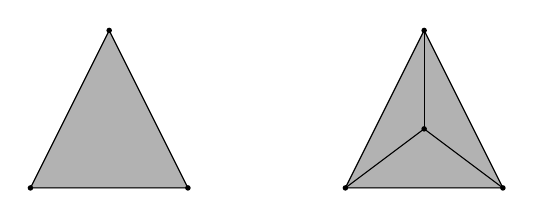
\begin{tikzpicture}[scale=1]
  % Coordinates
  \coordinate (A) at (0.00, 0.00);
  \coordinate (B) at (1.00, 2.00);
  \coordinate (C) at (2.00, 0.00);
  \coordinate (D) at (4.00, 0.00);
  \coordinate (E) at (5.00, 2.00);
  \coordinate (F) at (6.00, 0.00);
  \coordinate (G) at (5.00, 0.75);

  % Drawing
  \draw (A) -- (B) -- (C) -- cycle;
  \draw (D) -- (E) -- (F) -- cycle;
  \draw[fill,opacity=0.3] (A) -- (B) -- (C) -- cycle;
  \draw[fill,opacity=0.3] (D) -- (E) -- (F) -- cycle;
  \draw (G) -- (E);
  \draw (D) -- (G);
  \draw (F) -- (G);
  \fill[black] (A) circle (1pt);
  \fill[black] (B) circle (1pt);
  \fill[black] (C) circle (1pt);
  \fill[black] (D) circle (1pt);
  \fill[black] (E) circle (1pt);
  \fill[black] (F) circle (1pt);
  \fill[black] (G) circle (1pt);
\end{tikzpicture}\]
In the picture above, the two polyhedra are clearly the same (a triangle), but the complex on the left has a single face of dimension $2$, while the complex on the right has three.
\begin{definition}[Triangulation]
    Let $P$ be a polyhedron in $\R^n$. A simplicial complex $K$ such that $|K|=P$ is called a \textbf{triangulation} of $P$.
\end{definition}

In particular, starting from a single simplicial complex, we can generate arbitrarily rich simplicial complexes that all realize the same polyhedron.
\begin{definition}[Barycentric subdivision]
    Recall that if $\sigma=\set{\sum_{i=0}^k \alpha_i v_i\ |\ \alpha_i\in[0,1],\ \sum\alpha_i=1, v_i\in V}$, the point
    \[b_\sigma=\frac{1}{k+1}\sum_{i=0}^k v_i\]
    is called the \textbf{barycenter} of $\sigma$.

    Let $K=(V,\Sigma)$ be a simplicial complex. We call the \textbf{barycentric subdivision} of $K$ the simplicial complex $K^{(1)}$ having as vertices the set of barycenters of faces in $\Sigma$,
    \[V^{(1)}=\set{b_\sigma:\sigma\in\Sigma}\]
    and as simplices those obtained by inductively replacing vertices with barycenters, in decreasing order of dimension:
    \[\sigma^{(1)}_{j}=\set{\alpha_1 v_1+\cdots+\widehat{\alpha_j v_i}+\alpha_j b_{\sigma}+\cdots+\alpha_k v_k\ |\ \alpha_i\in[0,1],\ \sum\alpha_i=1}\]
\end{definition}
Visually, the barycentric subdivision of a triangle looks as follows:
\[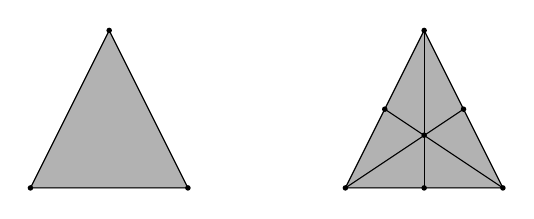
\begin{tikzpicture}[scale=1]
  % Coordinates
  \coordinate (A) at (0.00, 0.00);
  \coordinate (B) at (1.00, 2.00);
  \coordinate (C) at (2.00, 0.00);
  \coordinate (D) at (4.00, 0.00);
  \coordinate (E) at (5.00, 2.00);
  \coordinate (F) at (6.00, 0.00);
  \coordinate (G) at (5.00, 0.67);
  \coordinate (H) at (5.00, 0.00);
  \coordinate (I) at (5.50, 1.00);
  \coordinate (J) at (4.50, 1.00);

  % Drawing
  \draw (A) -- (B) -- (C) -- cycle;
  \draw (D) -- (E) -- (F) -- cycle;
  \draw[fill,opacity=0.3] (A) -- (B) -- (C) -- cycle;
  \draw[fill,opacity=0.3] (D) -- (E) -- (F) -- cycle;
  \draw (H) -- (E);
  \draw (D) -- (I);
  \draw (F) -- (J);
  \fill[black] (A) circle (1pt);
  \fill[black] (B) circle (1pt);
  \fill[black] (C) circle (1pt);
  \fill[black] (D) circle (1pt);
  \fill[black] (E) circle (1pt);
  \fill[black] (F) circle (1pt);
  \fill[black] (G) circle (1pt);
  \fill[black] (H) circle (1pt);
  \fill[black] (I) circle (1pt);
  \fill[black] (J) circle (1pt);
\end{tikzpicture} \]

\begin{theorem}[$|K|=|K^{(1)}|$]
    The geometric realization of a simplicial complex is unchanged by barycentric subdivision.
\end{theorem}
\begin{proof}
    We must show two inclusions: that $\sigma_j^{(1)}\subseteq \sigma$ for all $\sigma$ and all $j$, and that $\sigma\subseteq \bigcup_j\sigma^{(1)}_j$.

    For the first claim, suppose $p\in\sigma_j^{(1)}$; without loss of generality, $p\in \sigma_1^{(1)}$. Then
    \begin{align*}
        p&=a_1 b_\sigma + a_2 v_2+\cdots + a_kv_k\\
        &=\frac{a_1}{k+1}(v_1+\cdots+v_k)+a_2v_2+\cdots+a_kv_k\\
        &=\frac{a_1}{k+1} v_1+ (a_2+\frac{a_1}{k+1})v_2+\cdots+(a_k+\frac{a_1}{k+1})v_k.
    \end{align*}
    Now
    \begin{align*}
        &\frac{a_1}{k+1}+(a_2+\frac{a_1}{k+1})+\cdots+(a_k+\frac{a_1}{k+1})\\
        &=(k+1)\frac{a_1}{k+1}+a_2+\cdots+a_k\\
        &=a_1+a_2+\cdots+a_k=1,
    \end{align*}
    and all of these coefficients are positive. This means that any subdivision obtained by replacing a vertex with the barycenter of a face containing it, and taking the convex hull, is contained in the original face. Since the barycentric subdivision is an iteration of this process, $K^{(1)}\subseteq K$.

    For the converse, suppose $p\in \sigma$, so that
    \[p=a_1v_1+\cdots+a_kv_k.\]
    We want to find $b_1,\dots,b_k$ such that $p=b_1 v_1 + \cdots + b_j b_\sigma +\cdots + b_k v_k$. Substituting backwards,
    \begin{align*}
        &b_j v_j + b_1 v_1 + \cdots + b_k v_k\\
        &=\frac{a_j}{k+1} v_j + (a_1+\frac{a_j}{k+1}) v_1 + \cdots + (a_k+\frac{a_j}{k+1}) v_k,
    \end{align*}
    which yields the system of equations
    \[a_j=(k+1)b_j,\quad a_1= b_1-b_j, \quad \cdots, \quad a_k=b_k-b_j.\]
    To ensure that all the $b_i$ are positive, we choose $j$ to realize the minimum of the $b_j$.

    An induction on the subdivision then gives $K\subseteq K^{(1)}$.
\end{proof}
\subsection{Posets}
Forgetting the support in $\R^n$ gives a purely combinatorial description of a simplicial complex: what remains is essentially a downward-closed poset.
\begin{definition}[Face poset]
    Let $K=(V,\Sigma)$ be a simplicial complex. We call $[K]=(\Sigma,\subseteq)$ the \textbf{face poset} of $K$.
\end{definition}

The face poset $[K]$ already contains everything we need to recover the structure of $K$ up to PL-homeomorphism.
\begin{lemma}
    Let $K,K'$ be two simplicial complexes with $[K]\simeq [K']$. Then there exists a PL-homeomorphism $K\simeq K'$.
\end{lemma}
\begin{proof}
    See \cite[Lemma 2.18]{PLTopology}.
\end{proof}

This allows us to define:
\begin{definition}[ASC]
    An \textbf{abstract simplicial complex}, or \textbf{ASC}, is a pair $K=(V,\Sigma)$ where $V$ is a set and $\Sigma\subseteq \Pp(V)$ is a collection of subsets of $V$ closed under taking subsets.

    Given a simplicial complex $K$, associating to each face the set of its vertices yields an ASC $\overline{K}$.
\end{definition}

Conversely, every ASC arises this way from an essentially unique simplicial complex.
\begin{lemma}
    Let $K$ be an ASC. Then there exists a simplicial complex $K'$ such that $\overline{K'}=K$.
\end{lemma}
\begin{proof}
    Realize every $d$-simplex as the standard simplex of the appropriate dimension in $\R^{d+1}$, and glue them together according to their intersections; see \cite{PLTopology} for a complete account.
\end{proof}
Together, these two lemmas give a correspondence
\[\dfrac{\set{\textbf{Simplicial Complexes}}}{\text{PL-homeomorphism}}\leftrightarrow\set{\textbf{ASCs}}\]
since to each ASC we may associate a simplicial complex, and any two simplicial complexes associated to the same ASC are PL-homeomorphic.

We also want a way to define an (abstract) simplicial complex from any poset:

\begin{definition}[Nerve]
    Let $(P,\leq)$ be a poset. We call $\Nn(P)$, the \textbf{nerve} of $P$, the abstract simplicial complex whose vertices are the elements of $P$ and whose simplices are the flags $p_1<\cdots<p_k$ of ordered elements of $P$.
\end{definition}

We will freely use the following fact:
\begin{theorem}
    If $K=(V,\Sigma)$ is a simplicial complex, then
    \[\Nn(\Sigma)=\overline{K^{(1)}}.\]
\end{theorem}
\begin{proof}
    See \cite{PLTopology}.
\end{proof}
\subsection{Subdivision theorems}
We are interested in polyhedra as semantics for modal logic, and so our choice of morphisms differs slightly from the classical framework.

Recall first that, given (binary) Kripke frames $(W,R)$ and $(W',R')$, a function $f:W\to W'$ is called a p-morphism if and only if it satisfies
\begin{enumerate}
    \item $w R w'$ implies $f(w) R f(w')$;
    \item $f(v) R w'$ implies that there exists $w\in W$ such that $v R w$ and $f(w)=w'$.
\end{enumerate}

If $R=\leq$ is a partial order, these two conditions become equivalent to
\[\forall w\in W.\ \uparrow f(w)=f(\uparrow w),\]
where $\uparrow w=\set{v\in W: w<v}$. We refer to this property as \textbf{upward-closure}.

The proofs of all the following lemmas can be found in \cite{Dekker}.
\begin{lemma}[Subdivisions are p-morphic]
    The map $K^{(1)}\twoheadrightarrow K$ sending each face of $\Sigma^{(1)}$ to the (unique) face of $\Sigma$ containing it is a p-morphism.
\end{lemma}
\begin{lemma}[Common triangulation]
    Let $K$ be a simplicial complex and $K'\subseteq K$ another simplicial complex. Then there exists a subdivision $L$ of $K$, and a subset $L'$ of $L$ that is a subdivision of $K'$.
\end{lemma}
This is easy to visualize:
\[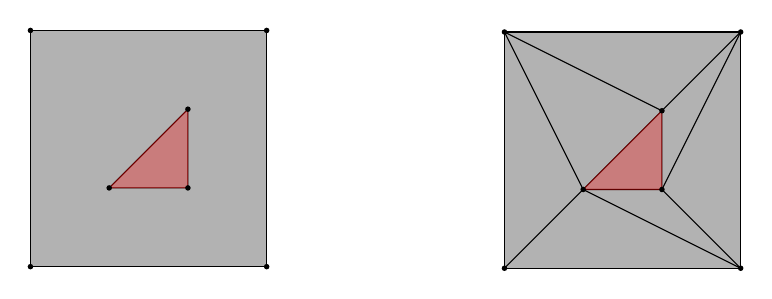
\begin{tikzpicture}[scale=1]
  % Coordinates
  \coordinate (A) at (0.00, 0.00);
  \coordinate (B) at (0.00, 3.00);
  \coordinate (C) at (3.00, 3.00);
  \coordinate (D) at (3.00, 0.00);
  \coordinate (E) at (1.00, 1.00);
  \coordinate (F) at (2.00, 2.00);
  \coordinate (G) at (2.00, 1.00);
  \coordinate (H) at (6.02, -0.02);
  \coordinate (I) at (6.02, 2.98);
  \coordinate (J) at (9.02, 2.98);
  \coordinate (K) at (9.02, -0.02);
  \coordinate (L) at (7.02, 0.98);
  \coordinate (M) at (8.02, 1.98);
  \coordinate (N) at (8.02, 0.98);

  % Drawing
  \draw (A) -- (B) -- (C) -- (D) -- cycle;
  \draw[fill, opacity=0.3] (A) -- (B) -- (C) -- (D) -- cycle;
  \draw (E) -- (F) -- (G) -- cycle;
  \draw[red,fill, opacity=0.3] (E) -- (F) -- (G) -- cycle;
  \draw (H) -- (I) -- (J) -- (K) -- cycle;
  \draw[fill, opacity=0.3] (H) -- (I) -- (J) -- (K) -- cycle;
  \draw (L) -- (M) -- (N) -- cycle;
  \draw[red,fill, opacity=0.3]  (L) -- (M) -- (N) -- cycle;
  \draw (H) -- (L);
  \draw (L) -- (K);
  \draw (N) -- (K);
  \draw (N) -- (J);
  \draw (M) -- (J);
  \draw (M) -- (I);
  \draw (L) -- (I);
  \fill[black] (A) circle (1pt);
  \fill[black] (B) circle (1pt);
  \fill[black] (C) circle (1pt);
  \fill[black] (D) circle (1pt);
  \fill[black] (E) circle (1pt);
  \fill[black] (F) circle (1pt);
  \fill[black] (G) circle (1pt);
  \fill[black] (H) circle (1pt);
  \fill[black] (I) circle (1pt);
  \fill[black] (J) circle (1pt);
  \fill[black] (K) circle (1pt);
  \fill[black] (L) circle (1pt);
  \fill[black] (M) circle (1pt);
  \fill[black] (N) circle (1pt);
\end{tikzpicture}\]

\begin{lemma}[Nerves are dense]
    Let $K$ be a simplicial complex and $L$ a subdivision of $K$.

    Then there exists $n\in \N$ such that $K^{(n)}$ is (isomorphic to) a subdivision of $L$.
\end{lemma}

\begin{lemma}[Subdividing p-morphisms]
    Let $K,K'$ be simplicial complexes and $f:K\upred K'$ an up-reduction, that is, a p-morphism defined on an upward-closed (open) subset of $K$.

    Let $L'$ be a subdivision of $K'$. Then there exists a subdivision $L$ of $K$ and an up-reduction $L\upred L'$ such that

    \[\begin{tikzcd}[ampersand replacement=\&]
	K \& {K'} \\
	L \& {L'}
	\arrow["\circ"{description, pos=0.17}, from=1-1, to=1-2, two heads]
	\arrow[from=2-1, to=1-1]
	\arrow["\circ"{description, pos=0.17}, from=2-1, to=2-2, two heads]
	\arrow[from=2-2, to=1-2]
\end{tikzcd}\]
\end{lemma}
